%%%%%%%%%%%%%%%%%%%%%%%%%%%%%%%%%%%%%%%%%
% Beamer Presentation
% LaTeX Template
% Version 1.0 (10/11/12)
%
% This template has been downloaded from:
% http://www.LaTeXTemplates.com
%
% License:
% CC BY-NC-SA 3.0 (http://creativecommons.org/licenses/by-nc-sa/3.0/)
%
%%%%%%%%%%%%%%%%%%%%%%%%%%%%%%%%%%%%%%%%%

%----------------------------------------------------------------------------------------
%	PACKAGES AND THEMES
%----------------------------------------------------------------------------------------

\documentclass[UTF8,aspectratio=169,14pt]{ctexbeamer}

\usepackage{hyperref}
\hypersetup{
	colorlinks=true,
	linkcolor=red,
	anchorcolor=blue,
	citecolor=green
}

\mode<presentation> {
	
	% The Beamer class comes with a number of default slide themes
	% which change the colors and layouts of slides. Below this is a list
	% of all the themes, uncomment each in turn to see what they look like.
	
	%\usetheme{default}
	%\usetheme{AnnArbor}
	%\usetheme{Antibes}
	%\usetheme{Bergen}
	%\usetheme{Berkeley}
	%\usetheme{Berlin}
	%\usetheme{Boadilla}
	%\usetheme{CambridgeUS}
	%\usetheme{Copenhagen}
	%\usetheme{Darmstadt}
	%\usetheme{Dresden}
	%\usetheme{Frankfurt}
	%\usetheme{Goettingen}
	%\usetheme{Hannover}
	%\usetheme{Ilmenau}
	%\usetheme{JuanLesPins}
	%\usetheme{Luebeck}
	\usetheme{Madrid}
	%\usetheme{Malmoe}
	%\usetheme{Marburg}
	%\usetheme{Montpellier}
	%\usetheme{PaloAlto}
	%\usetheme{Pittsburgh}
	%\usetheme{Rochester}
	%\usetheme{Singapore}
	%\usetheme{Szeged}
	%\usetheme{Warsaw}
	
	% As well as themes, the Beamer class has a number of color themes
	% for any slide theme. Uncomment each of these in turn to see how it
	% changes the colors of your current slide theme.
	
	%\usecolortheme{albatross}
	%\usecolortheme{beaver}
	%\usecolortheme{beetle}
	%\usecolortheme{crane}
	%\usecolortheme{dolphin}
	%\usecolortheme{dove}
	%\usecolortheme{fly}
	%\usecolortheme{lily}
	%\usecolortheme{orchid}
	%\usecolortheme{rose}
	%\usecolortheme{seagull}
	%\usecolortheme{seahorse}
	%\usecolortheme{whale}
	%\usecolortheme{wolverine}
	
	%\setbeamertemplate{footline} % To remove the footer line in all slides uncomment this line
	%\setbeamertemplate{footline}[page number] % To replace the footer line in all slides with a simple slide count uncomment this line
	
	%\setbeamertemplate{navigation symbols}{} % To remove the navigation symbols from the bottom of all slides uncomment this line
}

\usepackage{graphicx} % Allows including images
\graphicspath{{./figs/}}
\usepackage{booktabs} % Allows the use of \toprule, \midrule and \bottomrule in tables
\usepackage{longtable}
\usepackage{listings}
\usepackage{xcolor}
\lstset{numbers=left, %设置行号位置
	numberstyle=\tiny, %设置行号大小
	keywordstyle=\color{blue}, %设置关键字颜色
	commentstyle=\color[cmyk]{1,0,1,0}, %设置注释颜色
	frame=single, %设置边框格式
	escapeinside=``, %逃逸字符(1左面的键),用于显示中文
	%breaklines, %自动折行
	extendedchars=false, %解决代码跨页时,章节标题,页眉等汉字不显示的问题
	xleftmargin=2em,xrightmargin=2em, aboveskip=1em, %设置边距
	tabsize=4, %设置tab空格数
	showspaces=false %不显示空格
}
% Fonts
% \usepackage{libertine}
% \setmonofont{Courier}
\setCJKsansfont[ItalicFont=Noto Serif CJK SC Black, BoldFont=Noto Sans CJK SC Black]{Noto Sans CJK SC}


%----------------------------------------------------------------------------------------
%	TITLE PAGE
%----------------------------------------------------------------------------------------

\title[第3讲]{第3讲 中断、异常和系统调用} % The short title appears at the bottom of every slide, the full title is only on the title page
\subtitle{第四节:系统调用}
\author{向勇、陈渝} % Your name
\institute[清华大学] % Your institution as it will appear on the bottom of every slide, may be shorthand to save space
{
清华大学计算机系 \\ % Your institution for the title page
\medskip
\textit{xyong,yuchen@tsinghua.edu.cn} % Your email address
}
\date{\today} % Date, can be changed to a custom date

\begin{document}

\begin{frame}
\titlepage % Print the title page as the first slide
\end{frame}
%----------------------------------------------------------------------------------------
%\begin{frame}
%\frametitle{提纲} % Table of contents slide, comment this block out to remove it
%\tableofcontents % Throughout your presentation, if you choose to use \section{} and \subsection{} commands, these will automatically be printed on this slide as an overview of your presentation
%\end{frame}
%----------------------------------------------------------------------------------------
%	PRESENTATION SLIDES
%----------------------------------------------------------------------------------------

%------------------------------------------------
\section{第二节:系统调用}% Sections can be created in order to organize your presentation into discrete blocks, all sections and subsections are automatically printed in the table of contents as an overview of the talk

%----------------------------------------------
\begin{frame}[plain]	
	\frametitle{系统调用概貌}
	
	\begin{itemize}
		\item 应用程序要输出字符串时,会触发系统调用write()
	\end{itemize}\pause
	
	
	\centering
	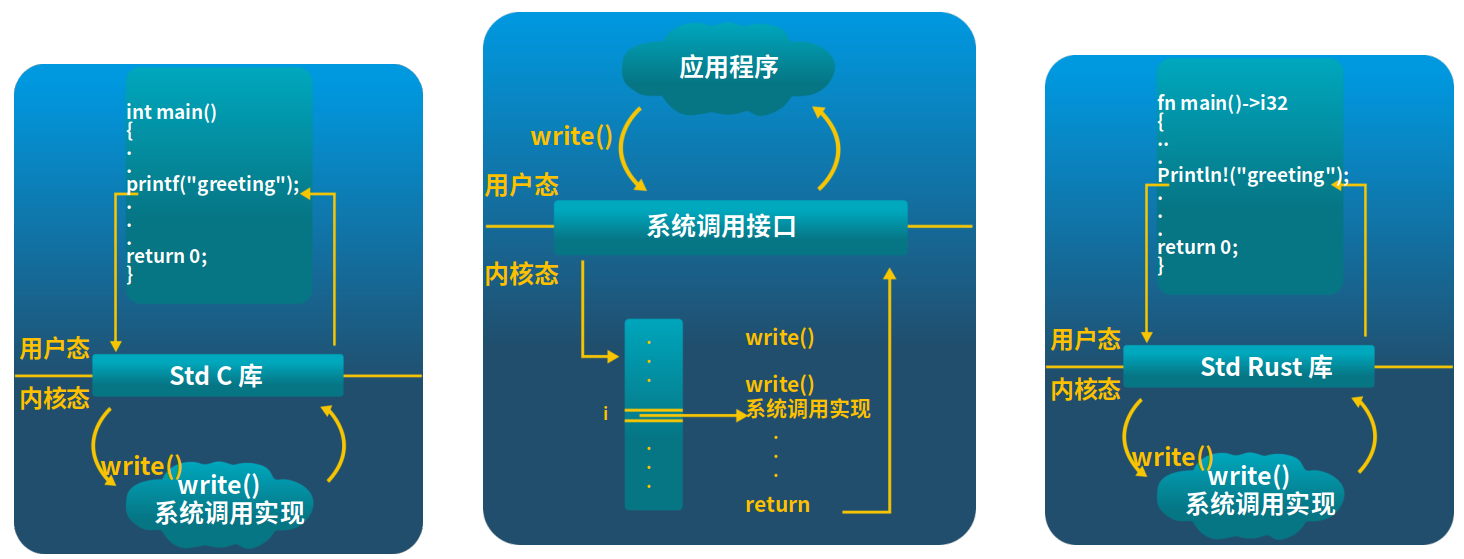
\includegraphics[width=1.\textwidth]{write-syscall}
	
\end{frame}


%------------------------------------------------
\begin{frame}
	\frametitle{系统调用概貌}
	
	
	\begin{columns}
		
		\begin{column}{0.4\textwidth}
			\centering
			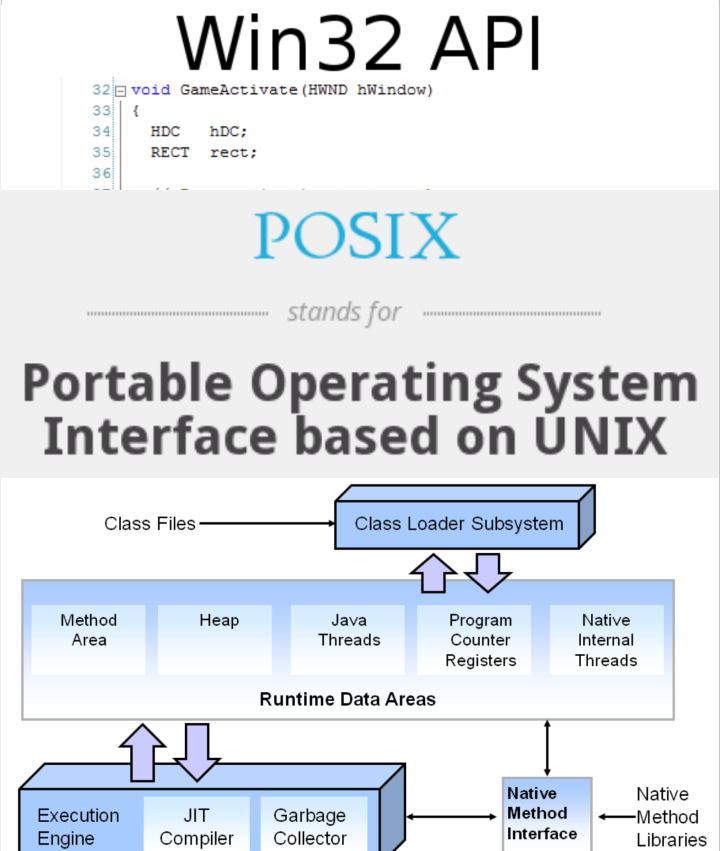
\includegraphics[width=1.0\linewidth]{syscalls}
			
			
		\end{column}
		
		\begin{column}{0.5\textwidth}
			
			\begin{itemize}
				\item 操作系统服务的应用编程接口
				\begin{itemize}
					\item 通常由高级语言编写(C、go和rust等)
					\item 程序通常访问高层次的API接口
				\end{itemize}\pause
				\item 三种最常用的应用程序编程接口
				\begin{itemize}
					\item Win API:用于 Windows 32/64
					\item POSIX API:用于 POSIX-based OS
					\item Java API:用于JAVA虚拟机(JVM)
				\end{itemize}
			\end{itemize}
			
		\end{column}
	\end{columns}
	
\end{frame}

%------------------------------------------------
\begin{frame}[plain]
	\frametitle{系统调用的实现概述}
	%	\framesubtitle{xxxx}
	\begin{columns}
		
		\begin{column}{0.45\textwidth}
			\centering
			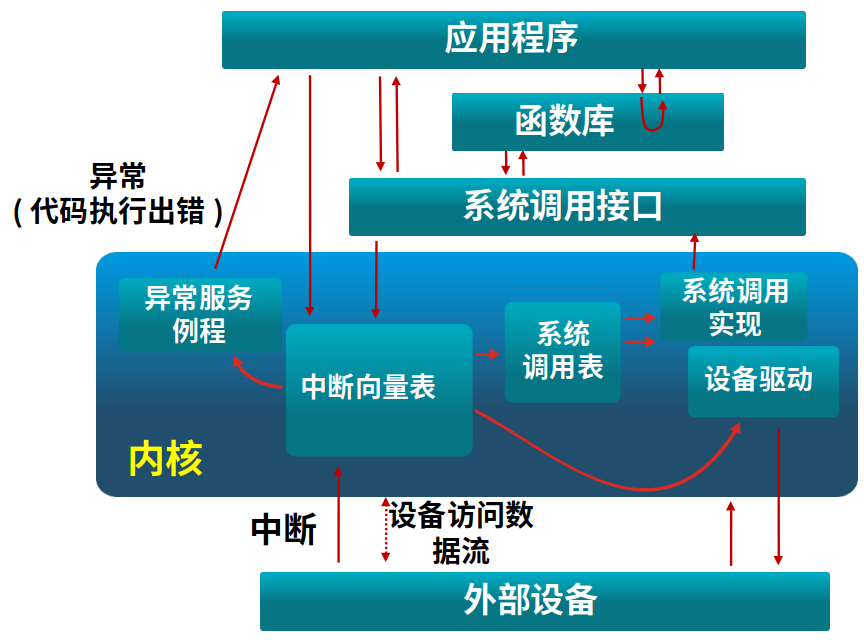
\includegraphics[width=1.0\linewidth]{os-4-intr-syscall-except}
			
		\end{column}
		
		\begin{column}{0.5\textwidth}
			
			\begin{itemize}  
				\item 用户态:通过运行库来管理 \pause
				\item 内核态:对应系统调用号
				\item 内核态:实现系统调用功能

				
			\end{itemize}
			
		\end{column}
		
	\end{columns}
	
\end{frame}


%------------------------------------------------
\begin{frame}[plain]
	\frametitle{函数调用和系统调用的不同处}
	%	\framesubtitle{xxxx}
	\begin{columns}
		
		\begin{column}{0.45\textwidth}
			\centering
			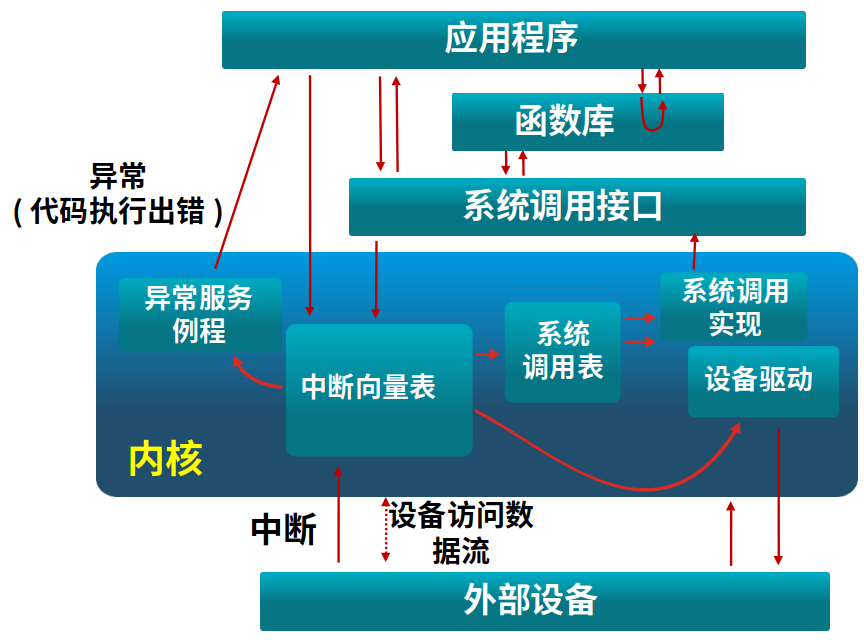
\includegraphics[width=1.0\linewidth]{os-4-intr-syscall-except}
			
		\end{column}
		
		\begin{column}{0.5\textwidth}
		
		  \begin{itemize}  
			\item 系统调用 \pause
			\begin{itemize}  
				\item RISC-V中,ecall和sret指令用于系统调用 \pause
				\item 堆栈切换和特权级的转换
			\end{itemize} \pause


			\item 函数调用
			\begin{itemize}  
				\item RISC-V中,call和ret指令用于系统调用
				\item 无堆栈切换和特权级的转换
			\end{itemize}	
			
			\end{itemize}			
		\end{column}
		
	\end{columns}
	
\end{frame}


%------------------------------------------------
\begin{frame}
	\frametitle{系统调用的开销}
%	\framesubtitle{xxxx}

	\begin{columns}
	
	\begin{column}{0.45\textwidth}
		\centering
		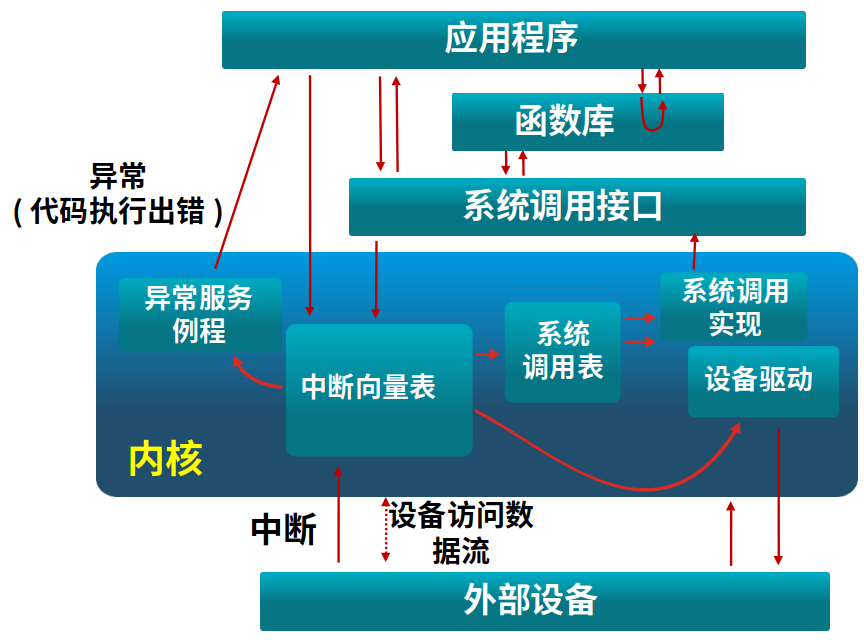
\includegraphics[width=1.0\linewidth]{os-4-intr-syscall-except}
		
	\end{column}
	
	\begin{column}{0.5\textwidth}
		
	\begin{itemize}
        \item 开销超过函数调用 \pause
        \item 开销:
	    \begin{itemize}

	        \item 切换内核堆栈
	        \item 验证参数
	        \item 可能切换页表
        	\item 需要拷贝书记

    	\end{itemize}
	\end{itemize}

	\end{column}

\end{columns}

\end{frame}


%------------------------------------------------
\begin{frame}[plain,t]
	\frametitle{系统调用机制--具体实现}
	%	\framesubtitle{xxxx}
	\begin{columns}
		
		\begin{column}{0.4\textwidth}
			\centering
			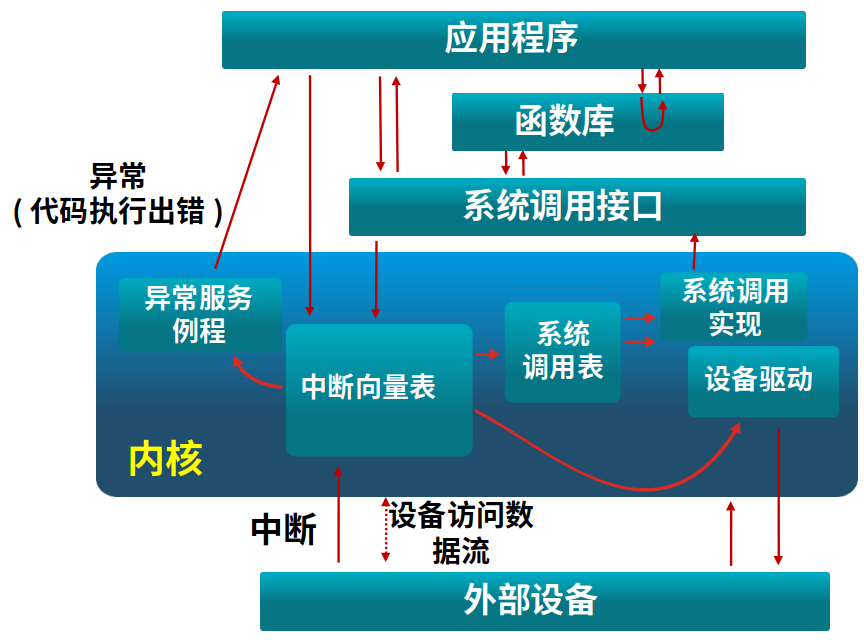
\includegraphics[width=1.0\linewidth]{os-4-intr-syscall-except}
			\begin{itemize} \small
				\item Core Local	Interruptor (CLINT)
				\item Platform-Level Interrupt Controller (PLIC)
			\end{itemize}
			
		\end{column}
		
		\begin{column}{0.5\textwidth}
			
%			\centering
			%			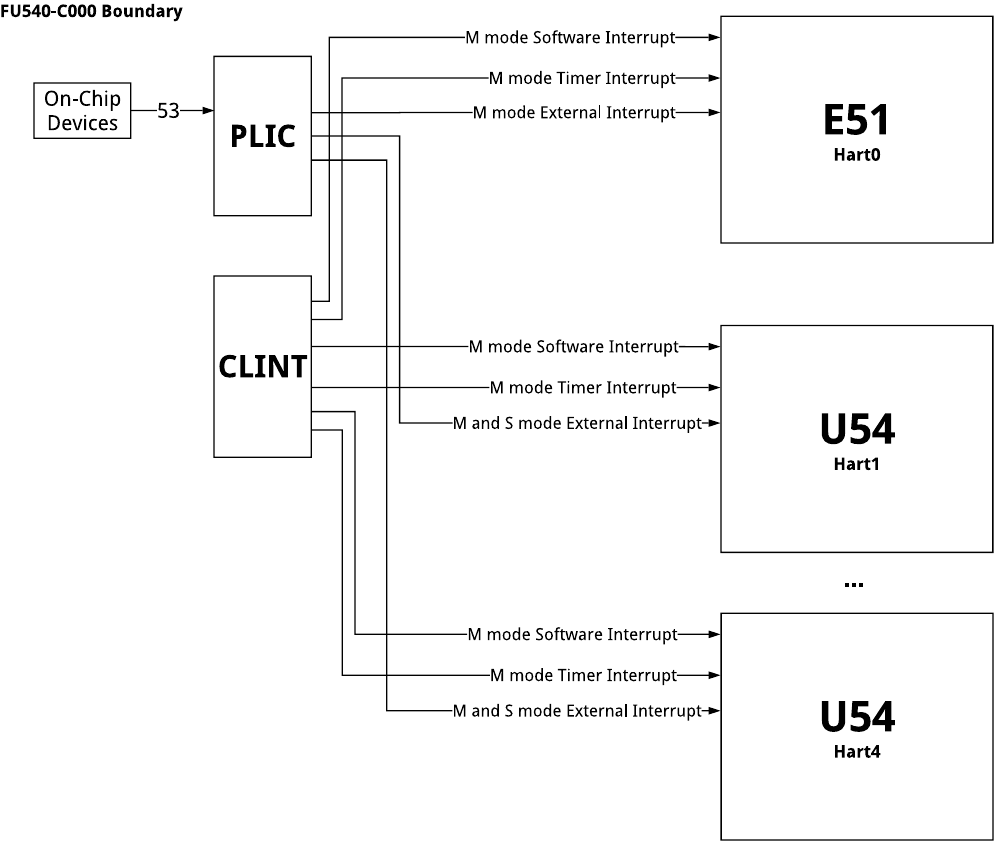
\includegraphics[width=.6\linewidth]{fu540-intr-arch}	
			%			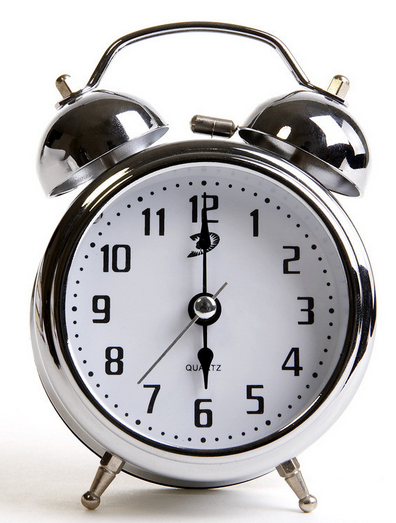
\includegraphics[width=.2\linewidth]{timer}
			%show rcore tutorial	
			应用发起请求  \pause
			\begin{itemize} \small 
				\item std lib 发出系统调用请求
				\begin{itemize} \small 
					\item 发出 设置系统调用号和参数,发出ecall	 

				\end{itemize} \pause				
				\item 硬件设置
				\begin{itemize} \small 
					\item sepc:保存请求后的指令地址	
					\item pc:设置为 stvec
					\item \underline{scause:设置为ecall from u-mode}
					\item sstatus:SIE位置零以禁用中断					
					\item stval:保存了相关的附加信息
				\end{itemize}  \pause
				\item 软件保存被打断现场\pause
				\item 执行软件实现的中断服务例程
				\item 软件恢复现场  \pause
				\item 应用继续执行
				
			\end{itemize}
			
		\end{column}
		
	\end{columns}
	
\end{frame}	

%----------------------------------------------------------------------------------------
\end{document}
